\chapter{Diskretes Äußeres Kalkül (DEC)}
\label{chapterDEC}

see \cite{Lee} \cite{FirstCourse}

\section{Diskrete Differentialformen}
  
  \begin{definition}
    Eine diskrete \( p \)-Form ist ein Homomorphismus vom Kettenkomplex \( C_{p}(K) \) nach \( \R \).
    Die Menge aller dieser Homomorphismen bezeichnen wir je nach Kontext mit \( C^{p}(K) \) (Menge der \( p \)-Koketten)
    oder \( \Omega^{p}_{d}(K) \) (Menge der diskrete \( p- \)(Differential-)Formen). 
    Das heißt
    \begin{align}
      \hom(C_{p}(K),\R) =: C^{p}(K) =: \Omega^{p}_{d}(K) \formpunkt
    \end{align}
    Desweiteren erfolgt die Addition punktweise, das heißt
    \begin{align}
      \left( \alpha + \beta \right)(c) &:= \alpha(c) + \beta(c)
    \end{align}
    für \( \alpha,\beta \in C^{p}(K) \) und \( c \in C_{p}(K) \).
  \end{definition}
  
  \begin{folgerung}
    \label{folgUnikKoketten}
    Da \( \R \) mit der Addition eine abelsche Gruppe ist, können wir uns wieder die Universalitätseigenschaft \eqref{diagFreieAbelscheGruppe} des Kettenkomplexes zunutze machen.
    Für eine \( p \)-Kette \( c = \sum_{\sigma\in K^{(p)}} a_{\sigma} \sigma \in C_{p}(K)\) und eine  \( p \)-Kokette \( \alpha\in C^{p}(K) \) gilt
    \begin{align}
      \alpha(c) &= \alpha\left(\sum_{\sigma\in K^{(p)}} a_{\sigma} \sigma\right) = \sum_{\sigma\in K^{(p)}} a_{\sigma} \alpha(\sigma) \formkomma
    \end{align}
    damit reicht es auch hier aus die \( p \)-Koketten nur auf den \( p \)-Simplizes zu definieren.
  \end{folgerung}

  Hätten wir die Menge der \( p \)-Ketten als \( \R \)-Vektoraum eingeführt, so hätte uns die Frage nach einem inneren Produkt zwischen den Ketten und den Koketten zur dualen Paarung
  geführt und damit auch, dass \( C^{p}(K) = \left( C_{p}(K) \right)^{*}\) der Dualraum von \( C_{p}(K) \) ist.
  Nun hält uns aber auch nichts davon ab, dies auch für die hier eingeführten Ketten analog zu machen.

  \begin{definition}
    \begin{align}
      \begin{aligned}
        \left\langle \bullet,\bullet \right\rangle : C^{p}(K) \times C_{p}(K)  &\rightarrow \R \\
                                                     \left( \alpha, c  \right) &\mapsto \left\langle \alpha, c \right\rangle := \alpha(c)
      \end{aligned}
    \end{align}
    heißt natürliche Paarung zwischen den \( p \)-Koketten (-Formen) und den \( p \)-Ketten.
  \end{definition}

  Die Verbindung zwschen diskreter Form und Differentialform ist die de-Rham-Abbildung.
  Dazu nehmen wir zunächst an, dass wir einen abstrakten Simplizialkomplex \( L \) vorliegen haben, das heißt, dass alle Simplizes auf der zugehörigen Mannigfaltigkeit \( M \) liegen.
  Das bringt erst einmal den Vorteil, dass Integration auf den Simplizes das gleiche Ergebinis auch auf der Mannigfaltigkeit liefert.

  \begin{definition}
    Die de-Rham-Abbildung bildet \( p \)-Differentialformen auf diskrete \( p \)-Formen (Koketten) ab. 
    Genauer
    \begin{align}
      \begin{aligned}
        \psi^{p}: \Omega^{p}(M) &\rightarrow C^{p}(L) = \Omega_{d}^{p}(L)\\
                       \alpha   &\mapsto \left( \sigma^{p} \mapsto \int_{\sigma^{p}} \alpha =: \psi^{p}(\alpha)(\sigma^{p}) =  \left\langle \psi^{p}(\alpha), \sigma^{p} \right\rangle\right)
                       \formkomma
      \end{aligned}
    \end{align}
    das heißt die diskrete \( p \)-Form \( \psi^{p}(\alpha) \in \Omega_{d}^{p}(L)  \) ist auf den \( p \)-Simplizes definiert, was wegen Folgerung \ref{folgUnikKoketten} vollkommen ausreicht.
  \end{definition}

  Da das Integral ein lineares Funktional ist, ist auch \( \psi \) linear.
  \todo{whitney abbildung noch ansprechen? Das heißt Interpolation im allgemeinen oder nur speziell?}

  \begin{bemerkung}
    Nun haben wir bei der Definition der de-Rham-Abbildung vorrausgesetzt, dass ein abstrakter Simplizialkomplex vorliegt.
    Das entspricht aber nur für flache Mannigfaltigkeiten unseren Anfoderungen.
    Im Allgemeinen ist die gegebene Triangulation nur eine lineare Approximation der Mannigfaltigkeit und damit auch des zugehörigen abstrakten Simplizialkomplexes.
    Das bedeutet auch, dass für \( p \ge 1 \) die Differentialformen von \( M \) in einem anderen Raum "`leben"' als die Differentialformen des Polytopes \( |K| \).
    Rein formal ließe sich die Situation entschärfen, in dem wir die Simplizes von \( K \) auf die Mannigfaltigkeit projizieren (vgl. \eqref{diagSingulaerAbstrakt}), also es wird
    \( \left\langle \psi^{p}(\alpha), \pi(\sigma^{p}) \right\rangle = \left( \psi^{p}(\alpha) \circ \pi \right)(\sigma^{p}) \) gerechnet für ein \( \sigma^{p}\in K \).
    Nur ist in vielen praktischen Aufgaben weder die Projektion noch die Mannigfaltigkeit exakt bekannt, so bleibt also nur die approximative Auswertung des Integrals auf den Ecken.
    Wir werden deshalb auch einfach  \( \left\langle \alpha_{d}, \sigma^{p} \right\rangle \) statt \( \left\langle \alpha_{d}, \pi(\sigma^{p}) \right\rangle \) schreiben.
    Für die numerische Analysis ist das eine schwierige Situation, da vor der eigentlichen Diskretisierung (Diskretisierungsfehler) noch eine Approximation (geometrischer Fehler) auf einen stückweise
    flachen Raum gemacht wird.

    Für \( 0 \)-Formen (identisch zu Skalarfeldern) ergibt sich dieser geometrische Fehler nicht, da nach Vorraussetzung die Ecken des Simplizialkomplexes auf der Mannigfaltigkeit liegen.
    Hier ist die Diskretisierung genauso wie wir das aus anderen Verfahren, wie die Finite-Differenzen-Methode, gewöhnt sind, da das "`Punktintegral"' nichts weiter als die Auswertung an
    eben diesem Punkt ist.
    Das heißt, liegt ein Skalarfeld \( u:M\rightarrow\R \) vor, so ist das diskrete Skalarfeld \( u_{d}:K^{(0)} \rightarrow \R \) an den Ecken definiert.
    \begin{align}
      u(v_{i}) &=  \psi(u)(v_{i}) = \left\langle \psi(u), v_{i} \right\rangle= u_{d}(v_{i}) =: u_{i} 
    \end{align}
    für alle \( v_{i} \in K^{(0)} \).
    Die Interpolation zurück zur Mannigfaltigkeit kann dann mittels linearer Ansatzfunktionen erfolgen, die sich auf den Volumenenelementen \( \sigma^{n} \) in gewohnter
    Weise definieren, das heißt 1 auf einer ausgezeichneten Ecke und 0 auf den übrigen Ecken.
    In dieser Arbeit werden wir uns auf die Auswertung von \( 0 \)-Formen beschränken, das reicht aus um skalarwertige oder vektorisierte skalarwertige Differentialgleichungen höherer
    Ordnung zu diskretisieren.

    Dennoch sei hier auf die Auswertung von \( 1 \)-Formen (Pfaffsche Formen) eingegangen, 
    denn sie werden zum einen für spätere numerischen Betrachtungen und zum anderen für die Behandlung von (Tangential-)Vektorproblemen
    noch interessant werden, denn mittels \( \flat \) beziehungsweise \( \sharp \) ist ein Isomorphismus zwischen Vektorfeldern und \( 1 \)-Formen gegeben.
    Betrachten wir hierzu eine \( 1 \)-Form \( \alpha\in\Omega^{1}(M) \) und die zugehörige diskrete Form \( \alpha_{d} = \psi(\alpha)\in\Omega^{1}_{d}(M) \).
    Wie sind diese beiden Formen zu vergleichen? 
    Beide geben haben zwar Antworten in \( \R \) aber die Differentialform nimmt einen Tangentialvektor und die diskrete Form eine Kante als Eingabe. 
    Dazu sei eine Kante \( \sigma^{1}_{\eps} \in K\) der Länge \( 2\eps \) gegeben und deren abstrakte Kante \( s_{\eps}\in L \), die auf der Mannigfaltigkeit liegt, 
    siehe Abbildung \ref{figDiskrete1Form}.
    \( s_{\eps}: (-\eps,\eps)\rightarrow M \) sei in Parameterform gegeben und zwar so, dass \( s_{\eps}(0)=x_{0}\in M \), \( \dot{s}_{\eps}(0) = v \in T_{x_{0}}M \) 
    und \( x_{0}\in M \subset \R^{N} \) so gewählt, dass \( v \) parallel zur Kante \( \sigma^{1}_{\eps} \) ist (Existenz folgt aus dem Mittelwertsatz der Differentialrechnung).
    Ohne Einschränkung der Allgemeinheit sei \( v \) der tangential Einheitsvektor in der umgebenen \( \xi \)-\( \eta \)-Ebene.
    Die Auswertung der diskreten Form an der Kante \( \sigma^{1}_{\eps} \) ergibt
    \begin{align}
        \alpha_{d}(\sigma_{\eps}^{1}) &= \langle \psi(\alpha) , s_{\eps} \rangle = \int_{s_{\eps}}\alpha = \int_{-\eps}^{\eps} (\alpha \circ \dot{s}_{\eps})(t) dt\\
                                 &\approx 2\eps \alpha(v) \formpunkt
    \end{align}
    Mit \( |\sigma^{1}_{\eps}| = 2\eps \) folgt 
    \begin{align}
      \frac{1}{|\sigma^{1}_{\eps}|} \alpha_{d}(\sigma_{\eps}^{1}) = \text{"`}\alpha_{d}(v)\text{"'} \approx \alpha(v)\formpunkt
    \end{align}
    \( \alpha_{d}(v) \) ist in Anführungszeichen gesetzt, da die diskreten Formen diese schreibweise nicht hergeben (\( v \cong \nicefrac{\sigma^{1}_{\eps}}{|\sigma^{1}_{\eps}|} \notin K \)), 
    aber wir wollen hier auf unnötigen Formalismus verzichten und uns ist
    klar was damit gemeint ist.
    Das Integral wurde an \( t=0 \) aproximiert, also mit der Mittelpunktsregel.
    Daher können wir abschätzen (siehe \cite{einfNum}, Kapitel 7)
    \todo{bei langeweile s mal explizit in lok.koords aufstellen um den Fehler besser abzuschätzen}
    \begin{align}
    \begin{aligned}
      \left| \text{"`}\alpha_{d}(v)\text{"'} - \alpha(v) \right|
              &\le \frac{(2\eps)^{3}}{24} \frac{1}{2\eps} \max_{\tau\in(-\eps,\eps)} \left|\frac{d^{2}(\alpha \circ\dot{s}_{\eps})}{dt^{2}}(\tau) \right| \\
              &= \frac{\eps^{2}}{6} \max_{\tau\in(-\eps,\eps)} \left|\frac{d^{2}(\alpha \circ \dot{s}_{\eps})}{dt^{2}}(\tau) \right| \formpunkt
    \end{aligned}
    \end{align}
    \begin{figure}
      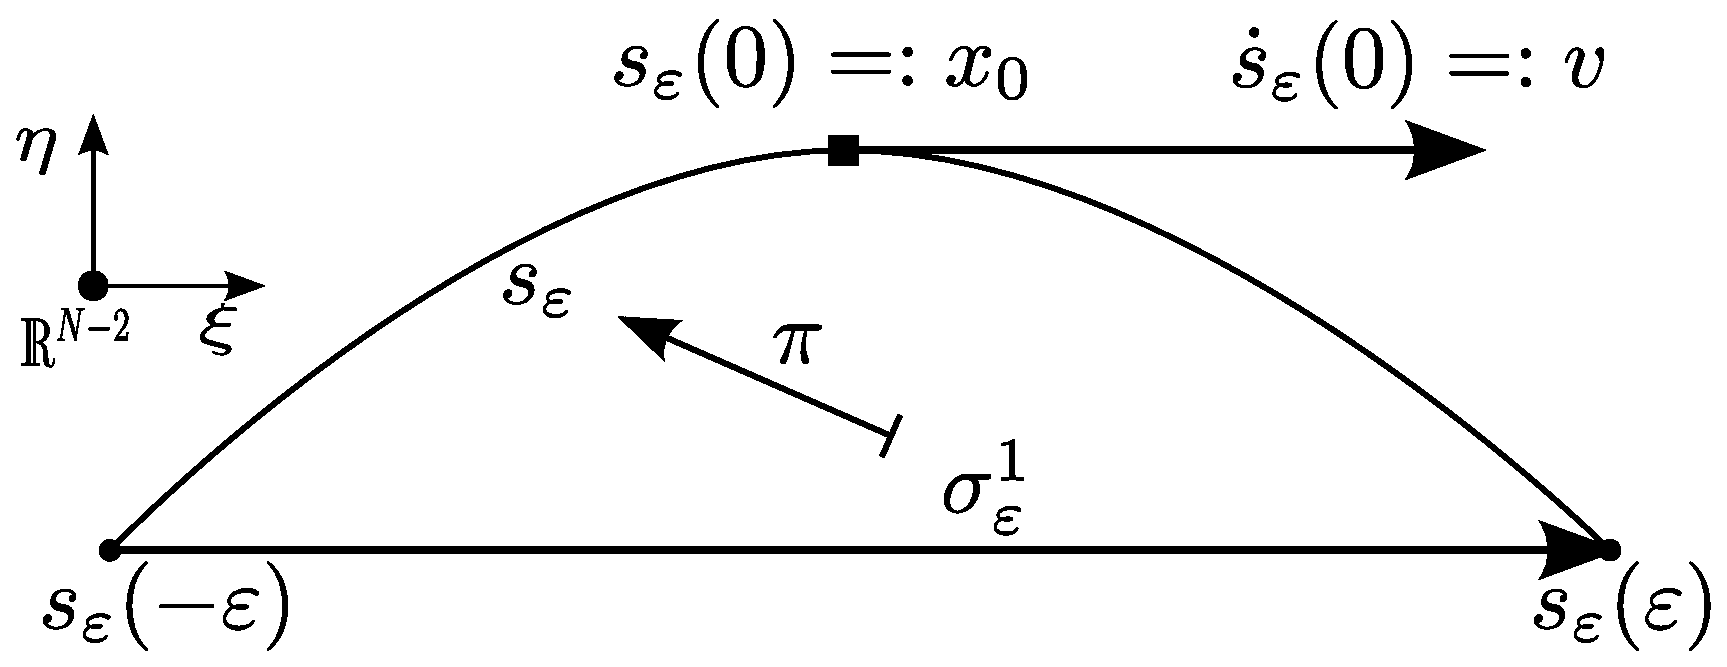
\includegraphics[width=\textwidth]{bilder/EpsilonKette.eps}
      \caption[Approximation einer 1-Form]{Das umliegende Koordinatensystem ist so gedreht, dass die Kante \( \sigma_{\eps}^{1} \) und die zugehörige abstrakte Kante \( s_{\eps} \)
                                           in der \( \xi \)-\( \eta \)-Ebene liegen. Die übrigen \( (N-2) \) Dimensionen zeigen aus der Bildebene heraus.
                                           \( \pi \) klebt die Kante auf die Mannigfaltigkeit, d.h. \( \pi(\sigma_{\eps}^{1}) = s_{\eps} \)}
      \label{figDiskrete1Form}
    \end{figure}
    Das soll nicht heißen, dass die \( 1 \)-Form \( \alpha\in\Omega^{1}(M) \) mit mindestens Ordnung 2 approximiert wird, denn im hinteren Faktor steckt noch immer die Größe \( \eps \).
    
    Dagegen lässt sich für exakte \( 1 \)-Formen tatsächlich eine Ordnung von 2 abschätzen.
    Sei eine exakte Form \( \alpha\in\Omega^{1}(M) \) gegeben, das heißt es existiert ein \( f\in\Omega^{0}(M) \), sodass \( \alpha= \exd f \) gilt.
    Mit dem Stokes Theorem (\cite{Marsden}, Kapitel 7.2) erhalten wir
    \begin{align}
    \label{eqExakt1FormPart1}
      \frac{1}{|\sigma^{1}_{\eps}|} \alpha_{d}(\sigma_{\eps}^{1}) &= \frac{1}{|\sigma^{1}_{\eps}|}\int_{s_{\eps}}\alpha 
                                                                   = \frac{1}{2\eps}\int_{\partial s_{\eps}} f
                                                                   = \frac{(f\circ s_{\eps})(\eps) - (f\circ s_{\eps})(-\eps)}{2\eps} \formpunkt
    \end{align}
    Wenn wir \( \left( x^{1},\ldots,x^{n} \right) \) als lokale Koordinaten der \( n \)-Mannigfaltigkeit am Punkt \( x_{0} \) wählen, 
    so dass \( x^{1} \) gerade die Standartkoordinate entlang der abstrakten Kante \( s_{\eps} \) ist mit \( v=\dot{s}_{\eps}(0) \) als tangentialer Einheitsvektor,
    also für die dualen Basisvektoren gilt 
    \begin{align}
      dx^{i}(v) &= \begin{cases}
                      1 & \text{falls } i=1 \\
                      0 & \text{sonst}
                  \end{cases} \formkomma
    \end{align}
    dann ergibt sich am Punkt \( x_{0}= s_{\eps}(0) \)
    \begin{align}
    \label{eqExakt1FormPart2}
      \begin{aligned}
        \alpha(v) &= \left( \exd f \right)(v) = \sum_{i=1}^{n}\frac{\partial f}{\partial x^{i}} dx^{i}(v)
                   = \nabla_{M}f \cdot v
                   = \nabla_{M}f \cdot \dot{s}_{\eps}
                   = \frac{d (f\circ s_{\eps})}{dt}(0) \formpunkt
      \end{aligned}
    \end{align}
    Da \eqref{eqExakt1FormPart1} nichts weiter als der Zentrale Differenzenquotient von \eqref{eqExakt1FormPart2} ist gilt
    \begin{align}
      \left| \text{"`}\alpha_{d}(v)\text{"'} - \alpha(v) \right| = \mathcal{O}(\eps^{2}) \formpunkt
    \end{align}

    Wir könnten nun auch ähnliche Betrachtungen für Differentialformen höheren Grades anstellen, jedoch werden wir uns im praktischen Teil nur auf zweidimensionale Oberflächen beschränken.
    Damit bleiben nur noch die \( 2 \)-Formen übrig und die unterscheiden sich wegen dem Hodge-Stern-Isomorphismus nur um einen geometrischen Faktor (und Syntax) von den \( 0 \)-Formen.
    Das heißt, wenn eine Riemannsche Mannigfaltigkeit vorliegt mit metrischen Tensor \( g \), dann gilt für alle \( 2 \)-Formen \( f \, dx^{1}\wedge dx^{2} \in \Omega^{2}(M)\), dass
    \begin{align}
      * \left( f \, dx^{1}\wedge dx^{2} \right) = \frac{f}{\sqrt{|\det(g)|}} \in \Omega^{0}(M) \formpunkt
    \end{align}
  \end{bemerkung}




  
  

\section{Äußere Ableitung}
  

  

  

\section{Hodge-Operator}

\section{Laplace-Operator}

  \subsection{Beispiel: Laplace-Gleichung}

  \subsection{Beispiel: Krümmung Teil 1: Gauß-Bonnet-Operator}
  \subsection{Beispiel: Krümmung Teil 2: Weingarten-Abbildung}
  \subsection{Beispiel: Krümmung Teil 3: Krümmungsvektor}


\section{Lie-Ableitung und Jacobian}

  \subsection{Beispiel: Wirbelgleichung}


